% --------------------------------------
% Document Class
% --------------------------------------
\documentclass[11pt]{article}
% --------------------------------------



% --------------------------------------
% Use Package
% --------------------------------------

% french, english
\usepackage[francais]{babel}

% font, french accent
\usepackage[utf8]{inputenc} 
\usepackage[T1]{fontenc} 

% page layout
\usepackage{geometry}

% hypertext link
\usepackage[pdfpagelabels]{hyperref}

\usepackage{graphicx}
\usepackage{float}
\usepackage{verbatim}
\usepackage{fancyhdr}
\usepackage{amsmath}


% include pdf
\usepackage[final]{pdfpages}


% --------------------------------------



% --------------------------------------
% Page setting
% --------------------------------------
%\pagestyle{empty}
\setlength{\headheight}{15pt}

\setcounter{secnumdepth}{3}
\setcounter{tocdepth}{2}

\makeatletter
\@addtoreset{chapter}{part}
\makeatother 

\hypersetup{         % parametrage des hyperliens
  colorlinks=true,      % colorise les liens
  breaklinks=true,      % permet les retours à la ligne pour les liens trop longs
  urlcolor= blue,       % couleur des hyperliens
  linkcolor= black,     % couleur des liens internes aux documents (index, figures, tableaux, equations,...)
  citecolor= green      % couleur des liens vers les references bibliographiques
}

% --------------------------------------

% --------------------------------------
% Information
% --------------------------------------
\title{Compte-rendu TP2 Rdf : Codage d'un contour}
\author{Elliot VANEGUE et Gaëtan DEFLANDRE}
% --------------------------------------



% --------------------------------------
% Begin content
% --------------------------------------
\begin{document}

  % Set language to english
  \selectlanguage{francais}

  % Start the page counting
  \pagenumbering{arabic}

  \maketitle
  
  \mbox{}
  \newpage
  \clearpage
  
  \section{Introduction}
  Lors de ce TP, nous allons utiliser différent algorithme permettant de déterminer
  les contours d'une forme afin de connaitre les avantages et inconvénient de chacun
  d'eux. Nous étudierons donc les descripteur de Fourier, ainsi que la l'algorithme
  de la corde.
  
  \section{Descripteurs de Fourier}
  Dans un premier temps nous allons calculer les descripteurs de Fourier. Pour cela
  Nous allons charger un fichier texte et calculer les descripteurs avec la méthode
  fft disponible dans le langage R. Nous pouvons voir que lorsque
  nous normalisons et que nous inversons les résultat de ce calcul, nous optenons
  à nouveau la position des points du contour.\\ 
  % TODO comment on le determine
  %On peut voir, suite à ces résultats
  %que le descripteur Z0 est le barycentre 
  
  Nous avons ensuite développé une méthode de filtrage des descripteur de Fourier dans
  le but de réduire le nombre de point pris en compte pour le calcul de ces descripteur.
  Nous remarquons que moins il y a de point, plus le carré se transforme en cercle.
  Cela se produit car nous perdons des details sur les descripteur de Fourier 
  lorsque nous réduisons le nombre de point.
  
  \begin{center}
    \begin{figure}[!h]
      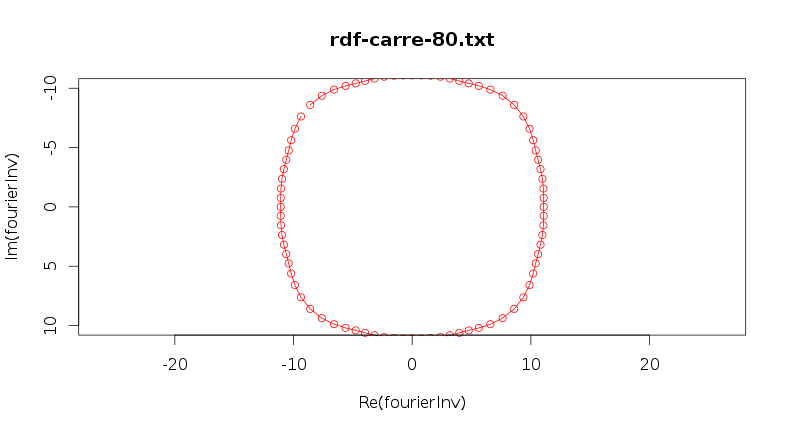
\includegraphics[width=15cm]{../resultat/carre-fourier-20.png}
      \caption{Image du carré avec 80\% des points supprimés}
    \end{figure}
  \end{center}
  
  Les descripteur de Fourier ne sont donc pas optimal si l'on veut déterminer le contour
  du forme rectangulaire.

  \section{Réduction d'une chaîne de contour}
  Cette algorithme de la corde va tracer des segments qui vont entourer une forme. Ces segments
  devront être le plus proche possible des contours de celle-ci. La distance entre ces segments
  et les points de la forme sera un paramètre que l'on pourra modifier afin d'avoir le niveau 
  de précisions qui convient le mieux. Sur une majorité des formes, plus on demandera une distance
  petite, plus l'algorithme devra calculer de points. Pour calculer cette distance, nous avons utiliser
  la formule suivante : 
  $abs(Im((cont - debut) * Conj(fin - debut))) / Mod(fin - debut)$.
  Cela nous a permit d'obtenir des contours plus ou moins précis en fonction du nombre
  de cette distance.
  
  \begin{center}
    \begin{figure}[!h]
      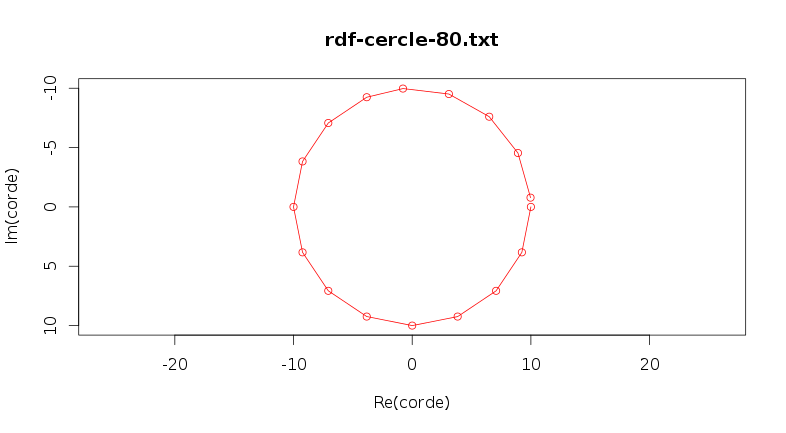
\includegraphics[width=15cm]{../resultat/cercle-corde-5.png}
      \caption{Image du cercle avec une distance maximum de 0.5 pixel}
    \end{figure}
  \end{center}
  
  \begin{center}
    \begin{figure}[!h]
      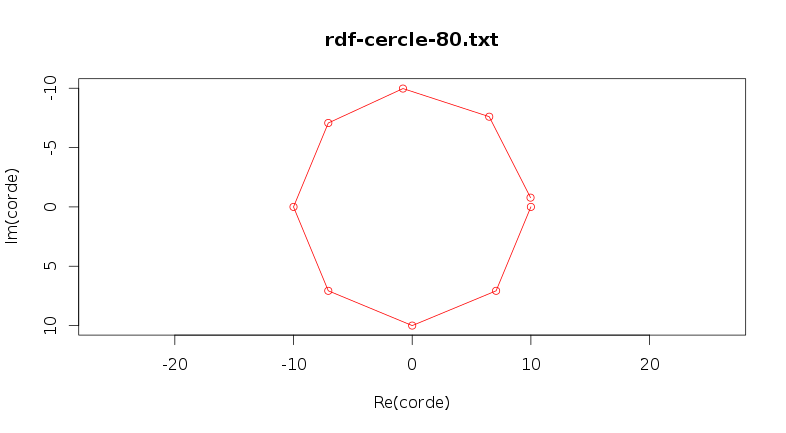
\includegraphics[width=15cm]{../resultat/cercle-corde-10.png}
      \caption{Image du cercle avec une distance maximum de 1 pixel}
    \end{figure}
  \end{center}
  
  Nous pouvons voir que cette algorithme reconnait assez bien la forme du cercle à la
  condition que la distance entre les points qui ont été déterminé et la corde soit assez
  petite. Ce qui implique qu'il faut calculer beaucoup de point pour avoir un résultat
  satisfaisant.\\
  
  Maintenant que nous savons calculer les descripteur de Fourier et utiliser l'algorithme
  de la corde nous allons comparer les résultat qu'ils fournissent sur différentes formes.
  
  \section{Comparaison des deux approches}
  Dans la suite de ce rapport, la courbe bleu représentera le tracé des descripteurs de Fourier
  et la courbe rouge le tracé de l'algorithme de la corde. 
  
   \begin{center}
    \begin{figure}[!h]
      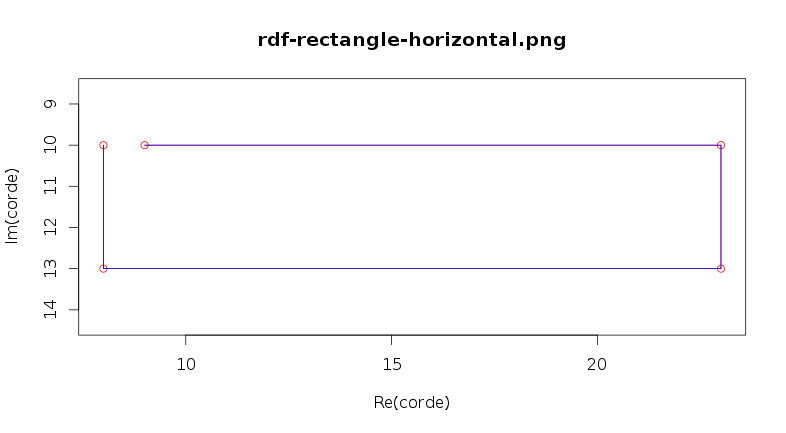
\includegraphics[width=15cm]{../resultat/comp_rect.png}
      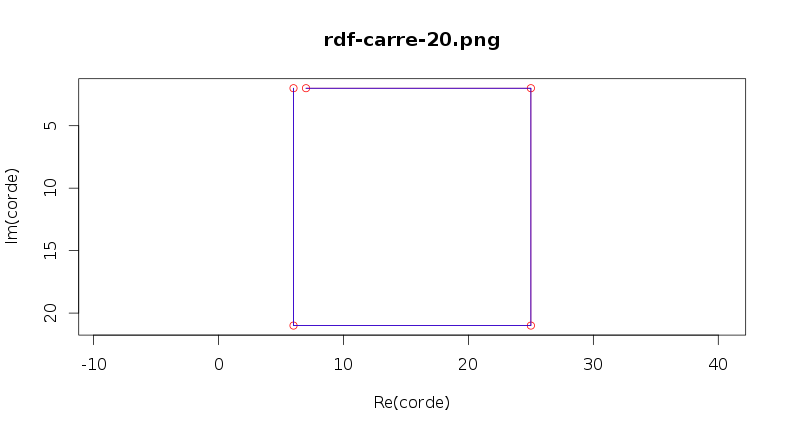
\includegraphics[width=15cm]{../resultat/comp_carre.png}
      \caption{Comparaison sur le rectangle horizontale et le carré: 100\% de descripteurs gardé et une distance de corde aléatoire}
    \end{figure}
  \end{center}
  
  \newpage
  %TODO
  Pour le rectangle et le carré, les deux méthodes sont aussi efficace l'un que l'autre. Cependant, l'algorithme de la corde
  fonctionne très bien avec un minimum de point à calculer.
  
  De plus, lorsque nous éliminons quelque descripteur de Fourier, l'algorithme n'est plus capable de 
  retrouver la forme, que se soit pour le rectangle ou le carré.\\
  
  \begin{center}
    \begin{figure}[!h]
      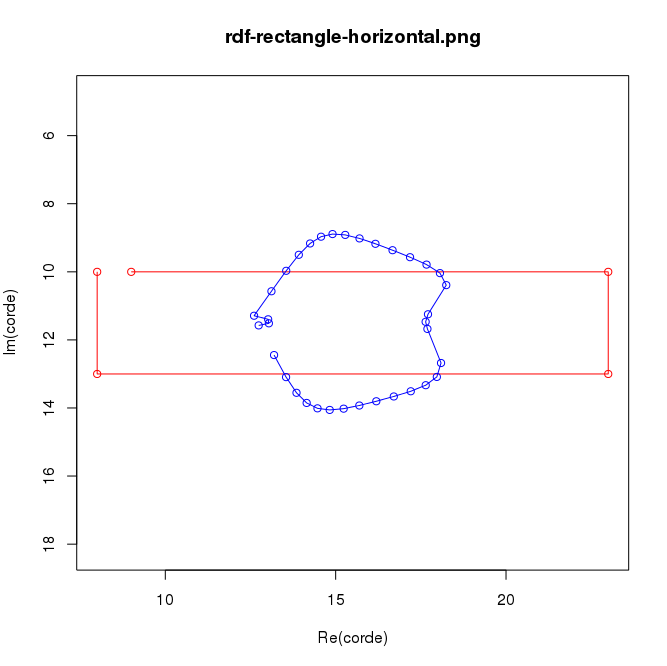
\includegraphics[width=15cm]{../resultat/comp_rate_rect.png}
      \caption{Comparaison sur le rectangle horizontale avec 90\% de descripteurs gardé}
    \end{figure}
  \end{center}
  
  Pour le triangle, le calcul des descripteurs de Fourier n'est pas très efficace même si nous gardons
  l'ensemble des descripteurs. L'algorithme de la corde quant à lui a besoin d'une distance minimal de 0.7 pixels pour
  reconnaitre parfaitement le triangle.
  
  \begin{center}
    \begin{figure}[!h]
      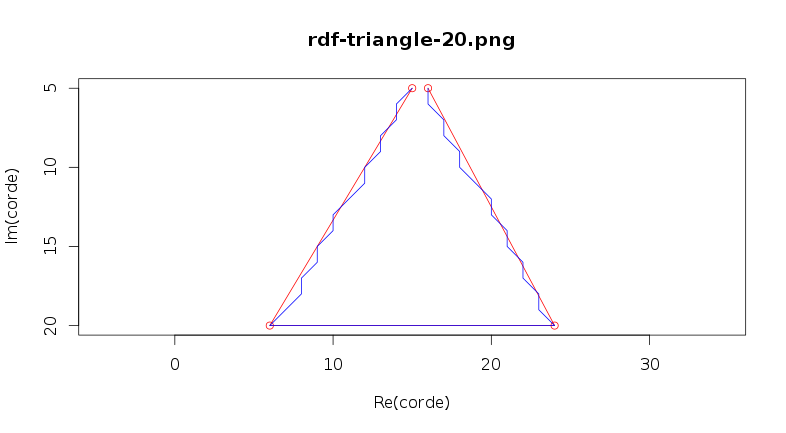
\includegraphics[width=15cm]{../resultat/comp_triangle.png}
      \caption{Comparaison sur le rectangle horizontale avec 90\% de descripteurs gardé}
    \end{figure}
  \end{center}
  
  \newpage
  
  Pour la croix, les observations sont les mêmes que pour le carré et le rectangle. Il faut tous
  les descripteurs de Fourier pour avoir un contour correcte et la distance pour l'algorithme de la 
  corde n'a pas d'importance.
  
  \begin{center}
    \begin{figure}[!h]
      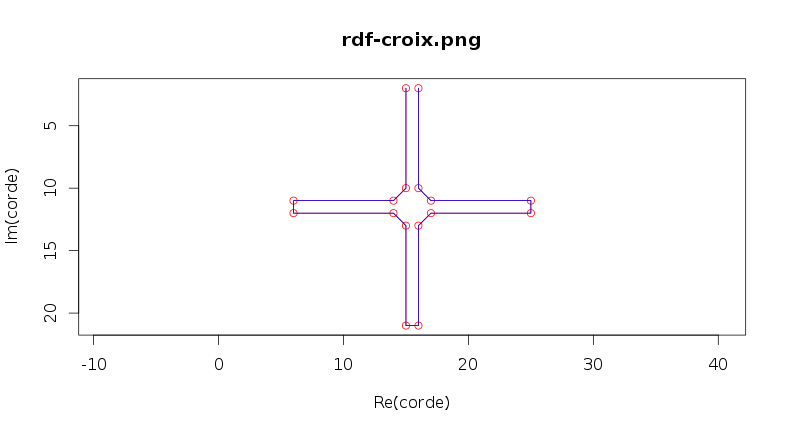
\includegraphics[width=15cm]{../resultat/comp_croix.png}
      \caption{Comparaison sur la croix}
    \end{figure}
  \end{center}
  
  \newpage
  
  Pour la patatoïde, les deux algorithmes sont efficaces mais la distance pour l'algorithme de la corde
  fait varier la précisions du contour. Pour un contour parfait il faut une distance de 0.1 pixels.
  
  \begin{center}
    \begin{figure}[!h]
      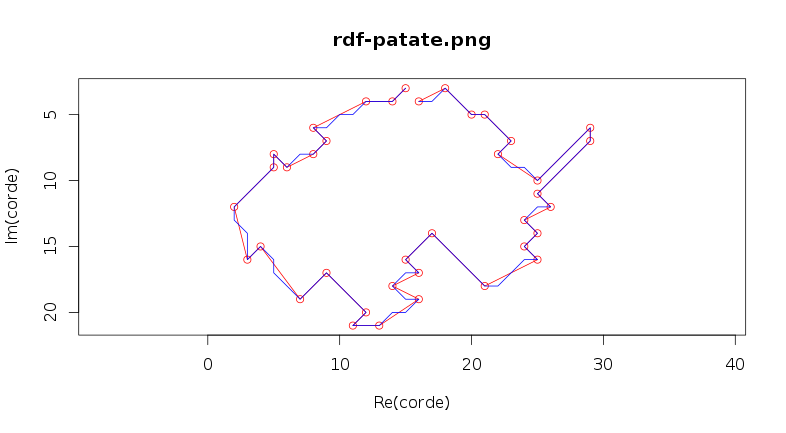
\includegraphics[width=15cm]{../resultat/comp_patate_impreci.png}
      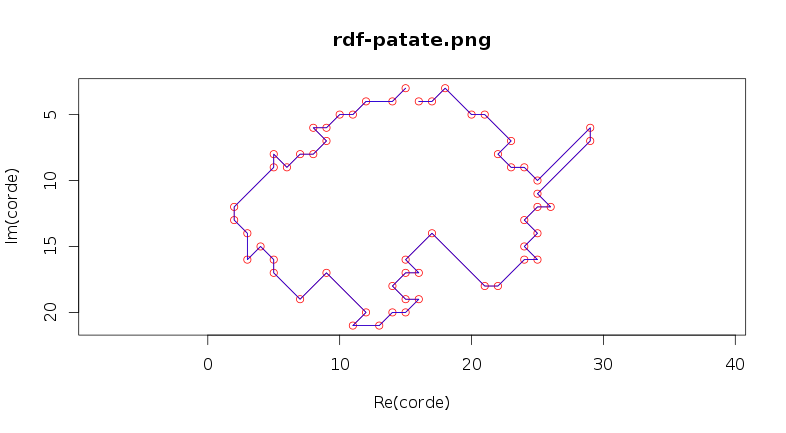
\includegraphics[width=15cm]{../resultat/comp_patate_preci.png}
      \caption{Comparaison sur la patate avec deux niveau de précisions pour l'algorithme de la corde}
    \end{figure}
  \end{center}
  
  \newpage
    
  \section{Conclusion}
  Suite au résultat que nous avons collecter précédement, on peut voir que les descripteurs de Fourier sont assez
  effication pour des formes circulaires où l'on peut même éliminer des descripteurs pour améliorer les performances
  de l'algorithme. Pour le reste des formes, il est efficace à condition d'avoir tous ses descripteurs. L'algorithme
  de la corde est très efficaces sur les formes rectangulaire où il a besoin de très peu de point pour obtenir un 
  contour parfait. Sur les formes arrondit par contre, il faut que la distance entre la corde et les points de la forme
  soit très petite pour que le contour soit bien reconnu.\\
  
  Donc l'algorithme de la corde est peut-être plus intéressant que le calcul des descripteurs Fourier car cette méthode
  peut-être très efficace avec un miminum de calcul sur certaine forme et sur les formes plus complexe il est au moins
  aussi efficace que la méthode de Fourier.
  
\end{document}